\chapter[流体力学]{\itr{Fluid Mechanics}{流体力学}}
\begin{solution}[\\A fluid is rotating at constant angular velocity $\omega$ about the central vertical axis of a cylindrical container.\\
    (a)Show that the \itr{variation}{变化} of pressure in the \itr{radial direction}{径向} is given by $\dfrac{\dif p}{\dif r}=\rho \omega^2 r$.\\
    (b)Take $p=p_c$ at the axis of rotation (r=0) and show that the pressure $p$ at any point $r$ is
    \[
        p=p_c+\dfrac{1}{2}\rho\omega^2 r^2
    \]
    (c)Show that the liquid surface is of \itr{paraboloidal}{抛物面的} form; that is, a vertical cross section of the surface is the curve $y=\dfrac{\omega^2 r^2}{2g}$]
    \begin{center}
    	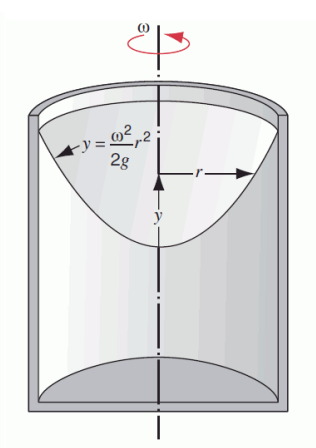
\includegraphics[width=0.45\textwidth]{chapter4_流体静力学}\\
    	\itshape 流体静力学
    \end{center}
    (a)取一段竖直方向的薄平面,设其截面积为A,沿半径方向的厚度为$\dif r$,深度为$h$。如下图所示:
    \begin{singlefigure}[A-4-1]{chapter4_E1_A1}[0.45]
    \end{singlefigure}

    可知水平方向的压强差为$\dif p=p_{r+\dif r}(h)-p_r(h)$,其中$p=p_0+\rho gh$。由受力关系结合匀速圆周运动可得:
        \[F=A\dif p=A\dif r \rho \omega^2 r\]
    整理得到(a)中的公式。
    
    (b)化简上式并积分:
        \[\int_{p_{h,0}}^{p_{h,r}}\dif p=\int_{0}^{r}\rho \omega^2 r\dif r\]

    得到:$p=p_0+\rho gh+\dfrac{\rho \omega^2 r^2}{2}$。其中前两项与半径无关,即为$p_c$,可得:
        \[p=p_c+\dfrac{1}{2}\rho \omega^2 r^2\]
        
    (c)液体表面的压强均为大气压强,将$p=p_0$、$p_c=p_0+\rho gh$代入(b)中得到的公式,得:
        \[\rho gh+\dfrac{1}{2}\rho \omega^2 r^2=0\]
    由于深度的坐标轴是向下的,我们以页面最低点处的水平方向为r轴,沿中心线竖直方向作为y轴,也就是调转一下坐标系。应用上述公式可知:
        \[y=\dfrac{\omega^2 r^2}{2g}\]
\end{solution}
\newpage
\begin{solution}[\\As shown in Figure 4-2, it is an \itr{air suction device}{空吸装置}. Given that the depth of the centerline of the \itr{catheter}{导管} below the liquid level in container $A$ is $h$, 
	the height difference between the liquid level in container $B$ and the centerline of the horizontal catheter is $h_b$, \itr{the cross-sectional area}{横截面积} at the \itr{nozzle}{喷嘴} $d$ is $S_d$, 
	and the cross-sectional area at the \itr{contraction section}{收缩段} $c$ is $S_c$. What are the conditions for the \itr{ratio}{比率} of $S_d$ to $S_c$ to occur for \itr{suction}{抽吸}?
    ]
    \begin{center}
    	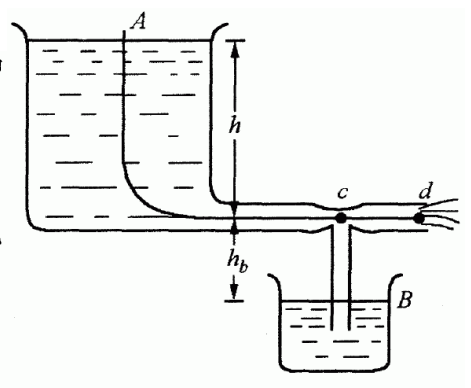
\includegraphics[width=0.65\textwidth]{chapter4_流体动力学}\\
    	\itshape 流体动力学
    \end{center}
    取一个流线Acd,对c、d两点应用伯努利公式可得:
        \[\dfrac{1}{2}\rho v_c^2+p_c=\dfrac{1}{2}\rho v_d^2+p_d\]
    其中d点的流速为$v_d=\sqrt{2gh}$,气压为大气压强$p_d=p_0$。且由于连续性原理,有:
        \[v_c S_c=v_d S_d\]
    因此c、d两点的压强差为:
        \[p_c-p_0=\rho gh(1-(\dfrac{S_d}{S_c})^2)\]
    而容器B液面的压强也是大气压强。发生空吸作用只要满足条件:
        \[p_c<p_0-\rho gh_b\]
    代入公式即可得到:
        \[\dfrac{S_d}{S_c}>\sqrt{1+(\dfrac{h_b}{h})}\]
\end{solution}